\section{Extension B: The virtual spectrometer (colour, prism, polarisation)}
Levels 1--4 give the lines of an atom in a field. This extension puts optics in front of them:
colours, a glass prism, polarisation filters, and the question of how fine an instrument must be.
The code lives in \texttt{src/optics/}.

\subsection{Three kinds of light and two viewing directions}
With $q = m_\text{upper} - m_\text{lower}$ the atom radiates $\pi$ light ($q=0$, a dipole along $\vb{B}$)
and $\sigma^\pm$ light ($q=\pm1$, a dipole rotating around $\vb{B}$). Their angular patterns share the
same total power:
\begin{equation}
  I_\pi(\theta)\propto \sin^2\theta,\qquad
  I_{\sigma}(\theta)\propto \tfrac12\,(1+\cos^2\theta),
\end{equation}
with $\theta$ the angle between the line of sight and $\vb{B}$.
\begin{table}[h]
\centering
\begin{tabular}{lll}
\toprule
& Across $\vb{B}$ ($\theta=90^\circ$) & Along $\vb{B}$ ($\theta=0^\circ$)\\
\midrule
$\pi$ & linear, parallel to $\vb{B}$, brightness 1 & absent\\
$\sigma^\pm$ & linear, perpendicular to $\vb{B}$, brightness $\tfrac12$ & circular, opposite handedness, brightness 1\\
\bottomrule
\end{tabular}
\caption{What each viewing direction shows, for equal emission rates.}
\end{table}

\subsection{Jones calculus for the filters}
Each component has a Jones vector $\vb{J}$ (basis: along the projection of $\vb{B}$ on the sky and
perpendicular to it). With time dependence $e^{-i\omega t}$,
$\vb{J}_\pi=(-\sin\theta,\,0)$ and $\vb{J}_{\sigma^\pm}=(\cos\theta,\ \pm i)/\sqrt2$, whose squared lengths are the
patterns above. An optical element is a $2\times2$ matrix $M$ and the observed intensity of a component is
\begin{equation}
  I_\text{obs} = R\;\lvert M\,\vb{J}\rvert^2,
\end{equation}
where $R$ is the component's emission rate. A linear polariser at angle $\varphi$ gives Malus's law,
and a quarter-wave plate followed by a polariser forms a circular analyser that passes $\sigma^+$ and blocks
$\sigma^-$ (or the reverse). Different lines are incoherent, so intensities add. Which handedness is
called ``left'' or ``right'' differs between textbooks and flips if $\vb{B}$ is reversed; the code states its
convention and the tests check consistency.

\subsection{Textbook intensity ratios, reproduced}
Viewed across the field in weak field the code gives, with nothing typed in by hand:
the four D1 components are equally bright, and the D2 components have relative intensities
$4:3:1$ (the two $\pi$ lines : the inner $\sigma$ pair : the outer $\sigma$ pair).
A polariser parallel to $\vb{B}$ keeps only the $\pi$ lines, one perpendicular keeps only the $\sigma$ lines,
and along the field a circular analyser splits the $\sigma^+$ lines from the $\sigma^-$ lines.

\begin{figure}[h]
\centering
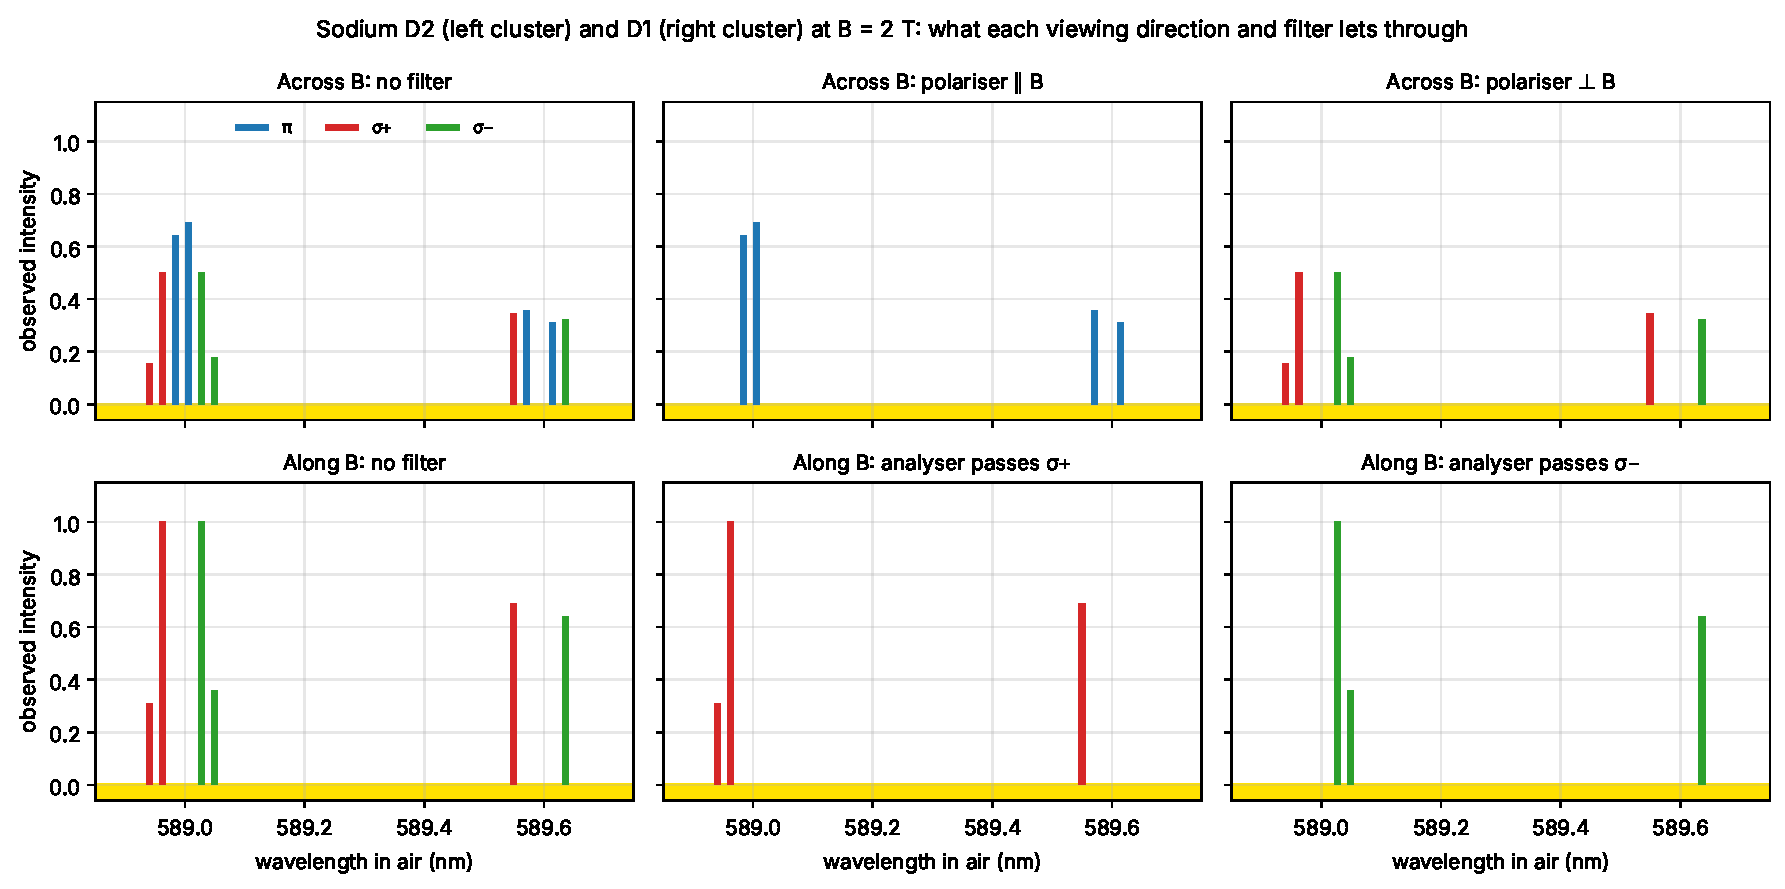
\includegraphics[width=\textwidth]{optics_polarisation_filters.pdf}
\caption{Sodium D lines at $B=2\ \si{T}$ through different filters and viewing directions.}
\end{figure}

\subsection{Colour and the prism}
A prism bends light by an amount set by $n(\lambda)$, which the code takes from the Sellmeier equation with
catalogue constants (BK7 reproduces $n_d=1.5168$). At minimum deviation
$\delta_\text{min}=2\arcsin(n\sin\tfrac A2)-A$. Violet bends most and red least, so a lamp spectrum spreads
into its colours on a screen (Figure~\ref{fig:prism}); the sodium D1 and D2 lines, only $0.6\ \si{nm}$ apart,
land close together.
\begin{figure}[h]
\centering
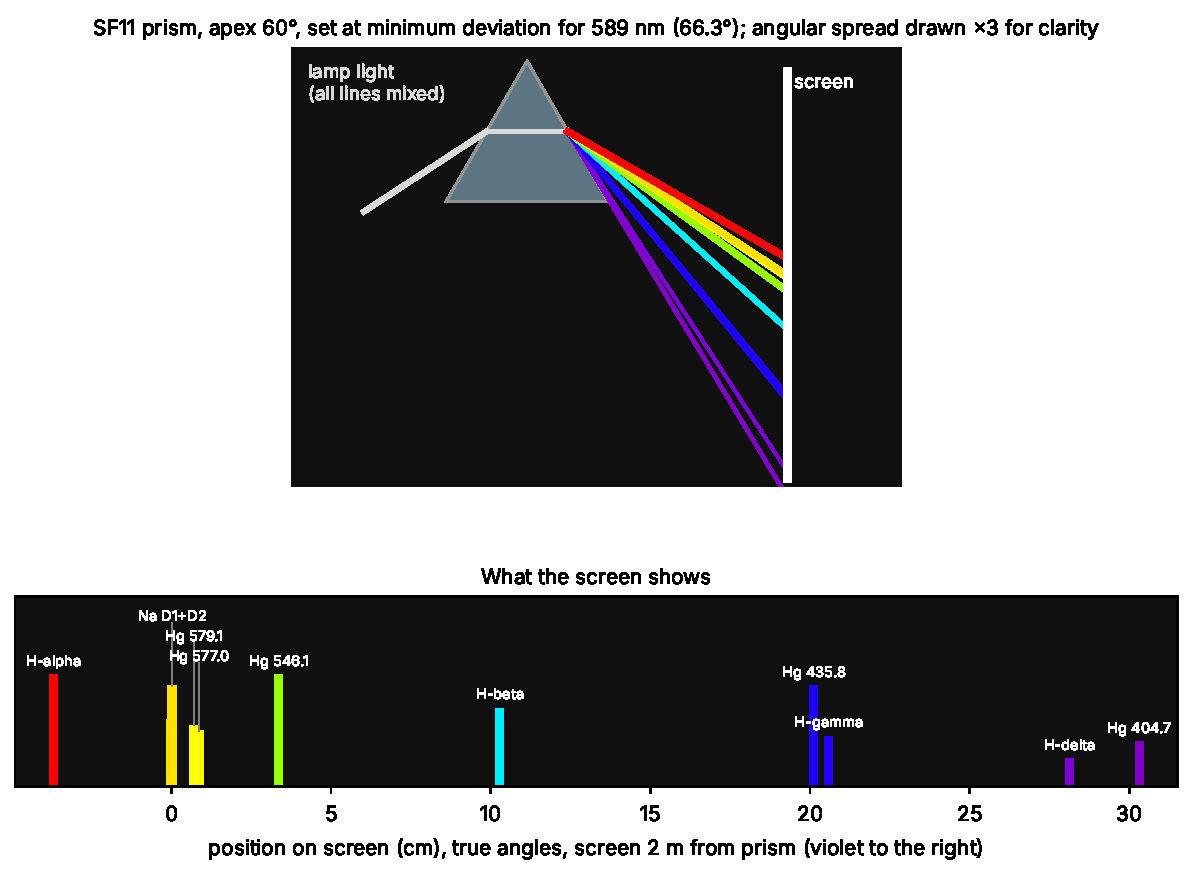
\includegraphics[width=0.85\textwidth]{optics_prism_setup.pdf}
\caption{A 60$^\circ$ SF11 prism splitting a lamp's lines (angular spread exaggerated $\times3$ in the ray drawing; the screen strip uses true angles).}
\label{fig:prism}
\end{figure}

\subsection{Can the prism show the Zeeman components?}
No. The outermost D2 component moves by only about $27\ \si{pm}$ per tesla, and all components are the same
yellow. The resolving power $R=\lambda/\Delta\lambda$ needed to separate the closest components is about
$5.5\times10^4$ at $1\ \si{T}$ and scales as $1/B$. Ideal resolving powers are about $2\times10^3$ for a 5\,cm BK7 prism,
$7.6\times10^3$ for SF11, $3\times10^4$ and $1.2\times10^5$ for gratings, and $10^6$ for a Fabry--Perot
(Figure~\ref{fig:ladder}). The weakest field at which each can just separate the components is $26$, $7.2$, $1.8$, $0.45$ and
$0.054\ \si{T}$ respectively; the BK7 prism needs about the crossover field $B^\ast=24.6\ \si{T}$, where the weak-field picture
has already ended.
\begin{figure}[h]
\centering
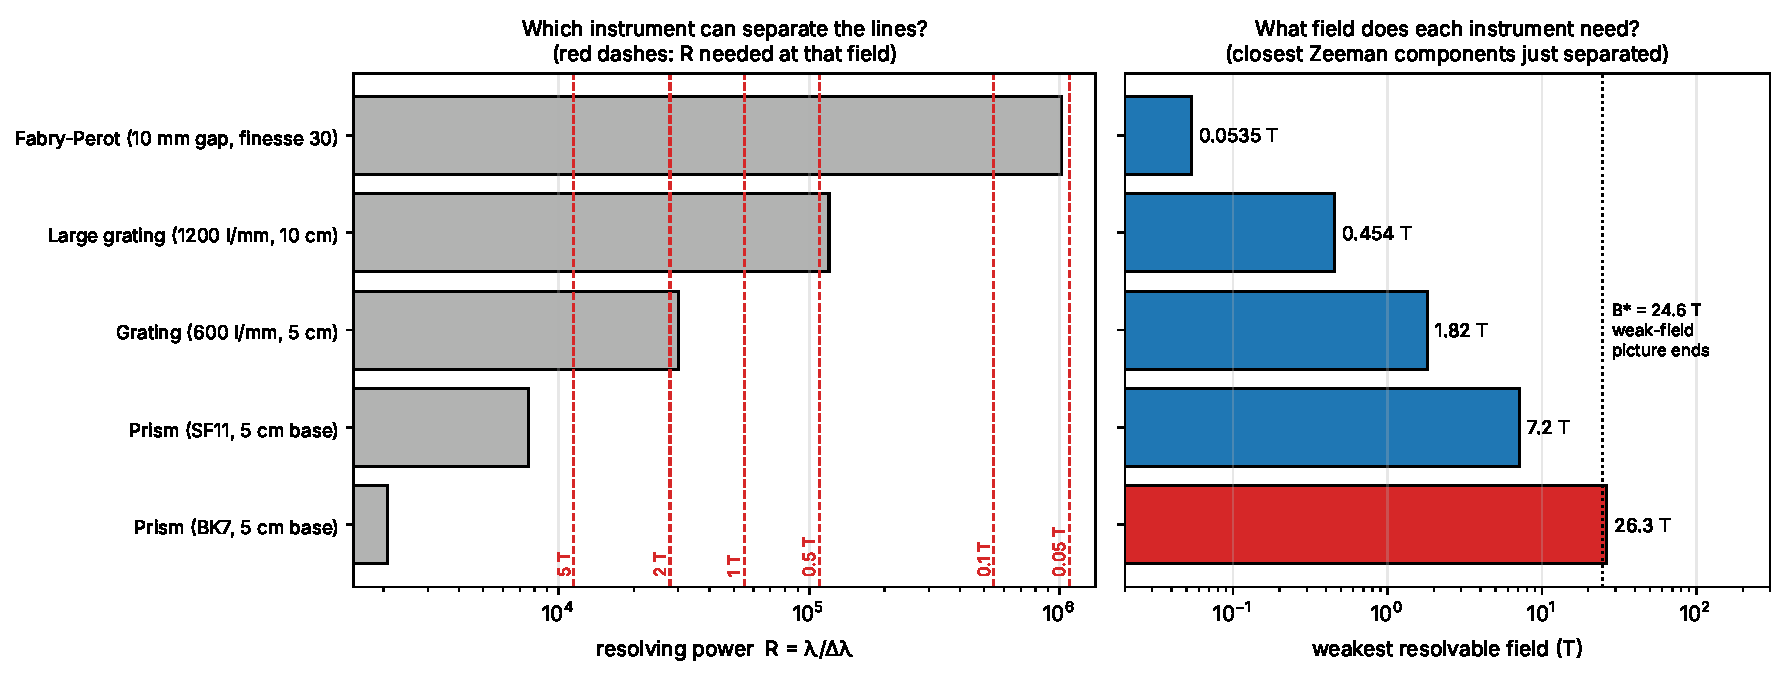
\includegraphics[width=\textwidth]{optics_instrument_ladder.pdf}
\caption{Instrument resolving powers (ideal) against the power the sodium Zeeman pattern needs.}
\label{fig:ladder}
\end{figure}
